% !TEX root = ../main.tex
\chapter{Especificación de Casos de Prueba (MVP) y Resultados}

\section{Especificación de Casos de Prueba (MVP)}
Para validar el incremento actual se definieron tres familias de pruebas: pruebas de funcionalidad, que verifican cada requisito funcional implementado de forma aislada sobre la API; pruebas de interfaz con usuarios reales, orientadas a garantizar la usabilidad del tablero; y pruebas de seguridad, centradas en los requisitos no funcionales críticos, en particular el almacenamiento seguro de credenciales del RNF-02. A continuación se presentan los casos correspondientes a las funcionalidades ya implementadas.

\subsection{Casos de prueba de funcionalidad}
Estos casos verifican el comportamiento esperado de cada endpoint implementado, mapeando cada prueba al requisito funcional que cubre.

\begin{longtable}{>{\bfseries}l >{\bfseries}l p{0.36\textwidth} p{0.38\textwidth}}
  \toprule
  ID & RF & Qué se prueba & Resultado esperado \\
  \midrule
  \endfirsthead
  \toprule
  ID & RF & Qué se prueba & Resultado esperado \\
  \midrule
  \endhead
  \bottomrule
  \caption{Casos de prueba de funcionalidad}
  \label{tab:cp_funcionalidad}
  \endfoot
  CP-01 & RF-04 & Creación de un tablero vacío. & El tablero se crea y aparece en el listado del usuario. \\
  CP-02 & RF-05 & Agregado de una tarjeta al tablero. & La tarjeta se crea y queda asociada al tablero en su posición inicial. \\
  CP-03 & RF-06 & Conexión de dos tarjetas mediante un hilo. & La strand se crea y queda persistida en el tablero. \\
  CP-04 & RF-06 & Conexión con una tarjeta inexistente. & La operación es rechazada, evitando hilos colgantes. \\
  CP-05 & RF-06 & Eliminación de una tarjeta conectada. & Se elimina la tarjeta y sus strands asociadas, sin afectar las demás. \\
  CP-06 & RF-07 & Ejecución de una integración predefinida (\texttt{dolar\_oficial}). & La tarjeta devuelve los datos esperados de la fuente externa. \\
  CP-07 & RF-07 & Integración predefinida sin un parámetro requerido. & Se reporta un error explícito por la variable faltante. \\
  CP-08 & RF-08 & Conexión a una API externa personalizada. & La tarjeta muestra el dato proyectado a partir de la respuesta. \\
  CP-09 & RF-08 & Conexión a una URL inválida. & La tarjeta reporta el error sin romper el resto del tablero. \\
  CP-10 & RF-09 & Lectura repetida dentro del intervalo de rate. & La segunda lectura se sirve del caché; al expirar el rate, se refresca. \\
\end{longtable}

\subsection{Casos de prueba con usuarios para validar la interfaz}
Estas pruebas se realizan en sesiones moderadas con usuarios de perfil técnico y no técnico, observando cómo completan tareas concretas sobre el tablero sin asistencia previa, con el fin de detectar problemas de usabilidad.

\begin{table}[H]
  \centering
  \renewcommand{\arraystretch}{1.2}
  \begin{tabularx}{\textwidth}{>{\bfseries}l X X}
    \toprule
    ID & Tarea del usuario & Métrica de éxito \\
    \midrule
    UX-01 & Crear un tablero y agregar una primera tarjeta. & La completa sin asistencia ni necesidad de documentación. \\
    UX-02 & Conectar dos tarjetas con un hilo. & Descubre el gesto del hilo por sí mismo. \\
    UX-03 & Cambiar la configuración de una tarjeta predefinida. & Lo logra en pocos segundos y sin errores irrecuperables. \\
    UX-04 & Conectar una tarjeta a una API personalizada (perfil técnico). & Logra mostrar un dato en un tiempo razonable. \\
    UX-05 & Recuperarse de una configuración con una URL inválida. & Identifica el error y lo corrige sin perder la tarjeta. \\
    \bottomrule
  \end{tabularx}
  \caption{Casos de prueba de interfaz}
  \label{tab:cp_ux}
\end{table}

\subsection{Casos de prueba de seguridad}
Estas pruebas validan el almacenamiento seguro de credenciales exigido por el RNF-02, así como los controles de acceso propios de un sistema multiusuario.

\begin{table}[H]
  \centering
  \renewcommand{\arraystretch}{1.2}
  \begin{tabularx}{\textwidth}{>{\bfseries}l X X}
    \toprule
    ID & Qué se prueba & Resultado esperado \\
    \midrule
    SEC-01 & Almacenamiento de las credenciales de una API personalizada. & Las credenciales no se guardan en texto plano en la base de datos. \\
    SEC-02 & Exposición de credenciales al cliente. & La configuración devuelta al frontend omite los valores sensibles. \\
    SEC-03 & Acceso de un usuario a un tablero ajeno. & El acceso es rechazado; solo el dueño y los colaboradores pueden verlo. \\
    SEC-04 & Ejecución de una expresión de proyección costosa. & El timeout aborta la query sin afectar al resto del proceso. \\
    \bottomrule
  \end{tabularx}
  \caption{Casos de prueba de seguridad}
  \label{tab:cp_seguridad}
\end{table}

\section{Resultados de Testing}
Se desarrollaron los tests unitarios, de integración y de punta a punta, con el objeto de corroborar la correcta implementación del sistema en base a las pruebas definidas. Se configuró un sistema de CI/CD para asegurar la consistencia del código fuente a medida que avanza el equipo. En la Tabla~\ref{tab:resultados_testing} se resumen los resultados de la última ejecución.

En el backend, la cobertura se calcula sobre los paquetes propios, excluyendo los adaptadores de MongoDB y Redis, que se validan con 52 pruebas de integración ejecutadas contra instancias reales de ambas bases y un servidor OAuth2 simulado. Las suites del backend y del servicio de tiempo real se ejecutan automáticamente en GitHub Actions ante cada cambio, mientras que las del frontend se ejecutan de forma local.

\begin{table}[H]
  \centering
  \renewcommand{\arraystretch}{1.2}
  \begin{tabularx}{\textwidth}{>{\bfseries}l X r l}
    \toprule
    Servicio & Tipo de pruebas & Tests & Cobertura \\
    \midrule
    Backend (Go) & Unitarias y de controladores & 474 & 81,7 \% de sentencias \\
    Backend (Go) & Integración con MongoDB, Redis y OAuth2 simulado & 52 & No aplica \\
    Tiempo real (Node.js) & Unitarias & 19 & 97,5 \% de líneas \\
    Frontend (SvelteKit) & Unitarias de módulos y lógica & 91 & 39,3 \% de sentencias \\
    Servidor MCP (xmcp) & Sin pruebas automatizadas & 0 & No aplica \\
    \bottomrule
  \end{tabularx}
  \caption{Resultados de las pruebas automatizadas por servicio}
  \label{tab:resultados_testing}
\end{table}

Las pruebas de usabilidad se desarrollaron con un grupo selecto de personas, siguiendo el modelo de usuarios representativos. Se construyó un diseño preliminar de la web en Figma, y a partir de la misma se iteró con los usuarios hasta conseguir un nivel de éxito aceptable según el equipo.

\section{MVP en producción y vistas de la interfaz}
El desarrollo se encuentra actualmente en producción, disponible desde la url del sitio web. Se compró un dominio para la entrega final, con el objeto de hacer más fácil de recordar el nombre del producto y la url.

\begin{itemize}
  \item \textbf{Link a la web:} \url{https://corcheria.company/}
  \item \textbf{Link al repo de bitbucket:} \url{https://bitbucket.org/itba/pf-2026a-tablero-informacion-universal/src/main/}
  \item \textbf{Link al repo de Github:} \url{https://github.com/Tobias-Noceda/tablero-informacion-universal}
\end{itemize}

El acceso a la aplicación comienza con el inicio de sesión, que admite correo y contraseña o una cuenta de Google, y con el registro de nuevos usuarios, quienes deben verificar su correo antes de ingresar (RF-01 y RF-02). Las Figuras~\ref{fig:ui_login} y \ref{fig:ui_registro} muestran ambas pantallas.

\begin{figure}[H]
  \centering
  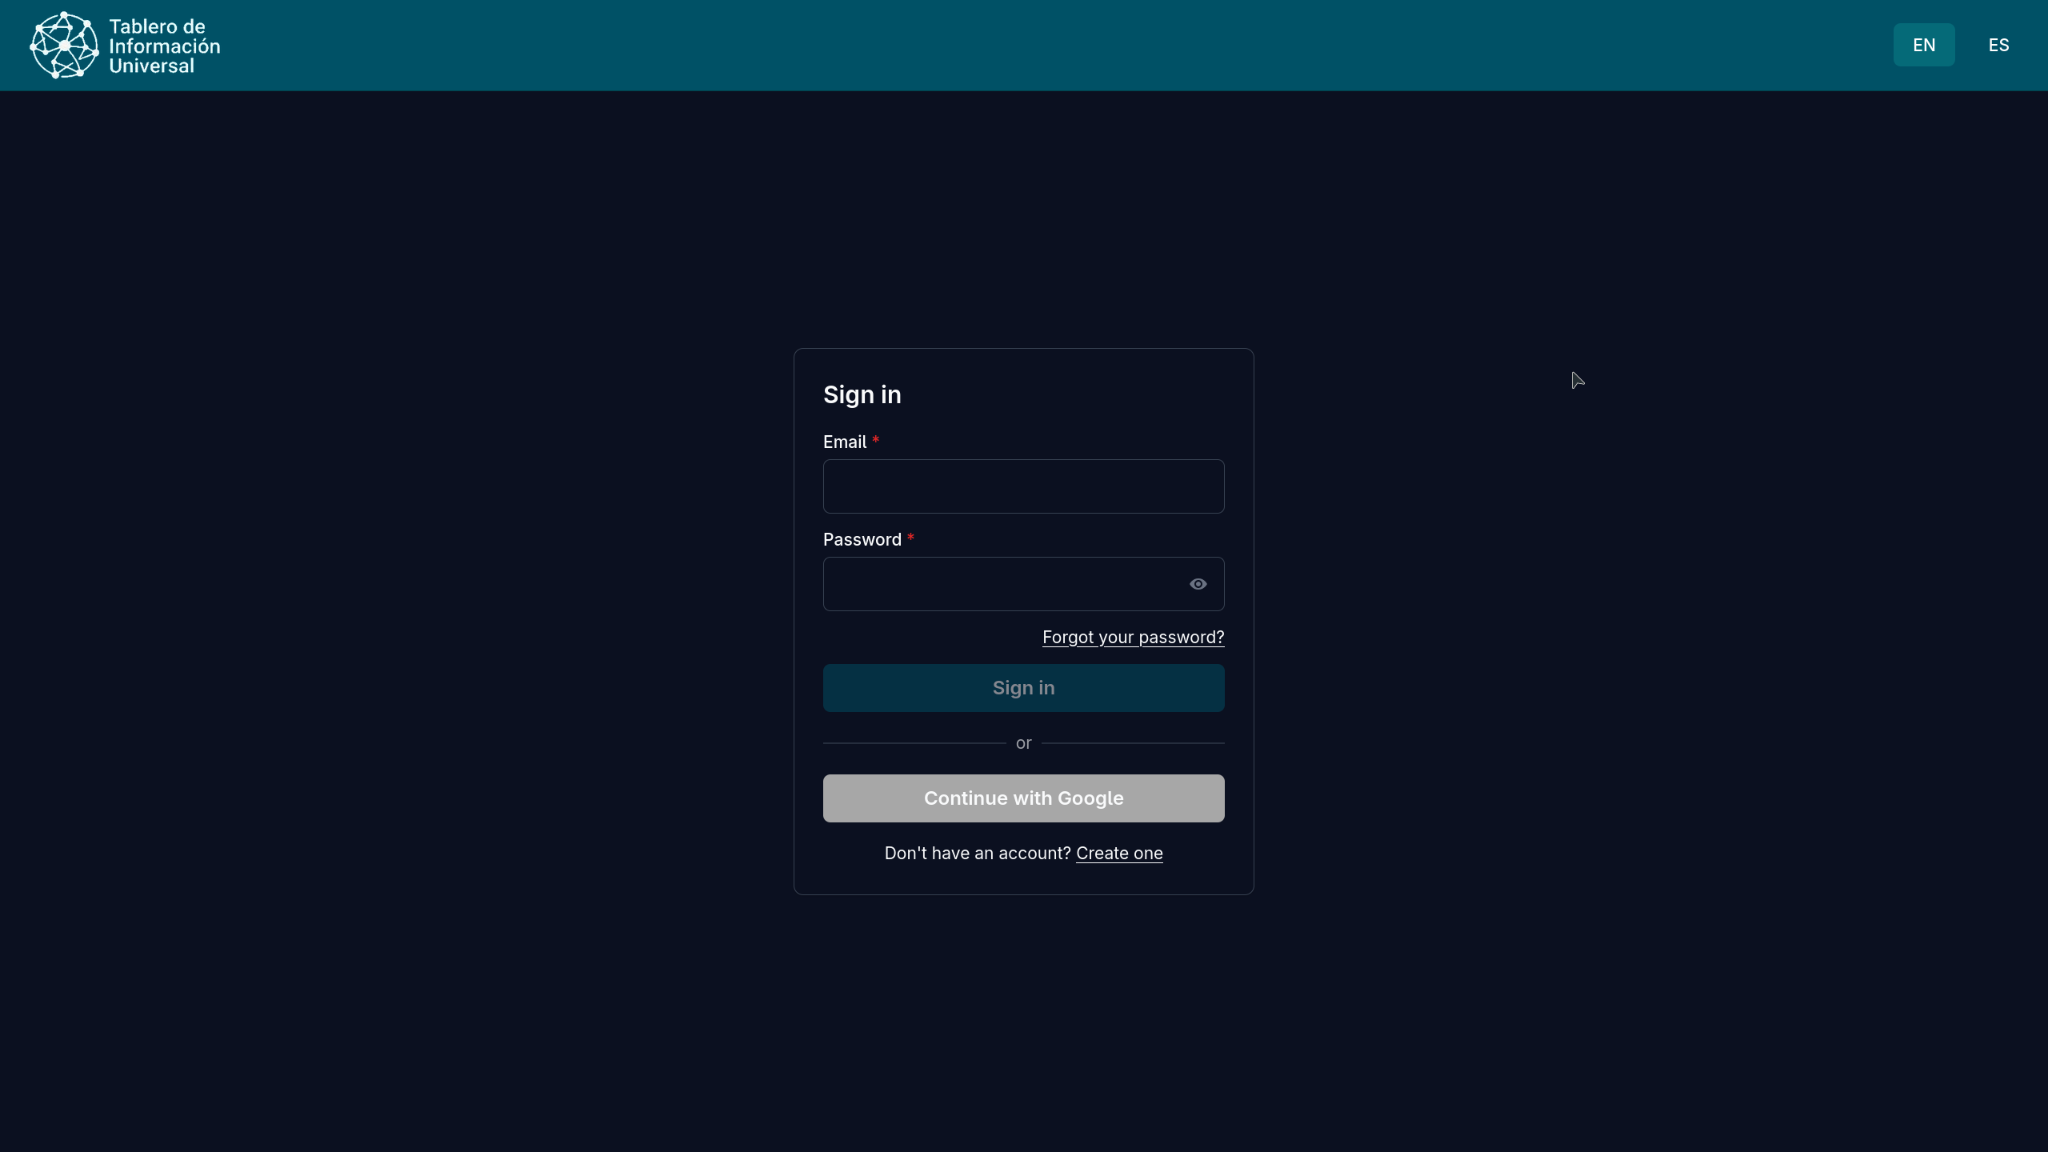
\includegraphics[width=0.92\textwidth]{figuras/fig28.png}
  \caption{Inicio de sesión en la web}
  \label{fig:ui_login}
\end{figure}

\begin{figure}[H]
  \centering
  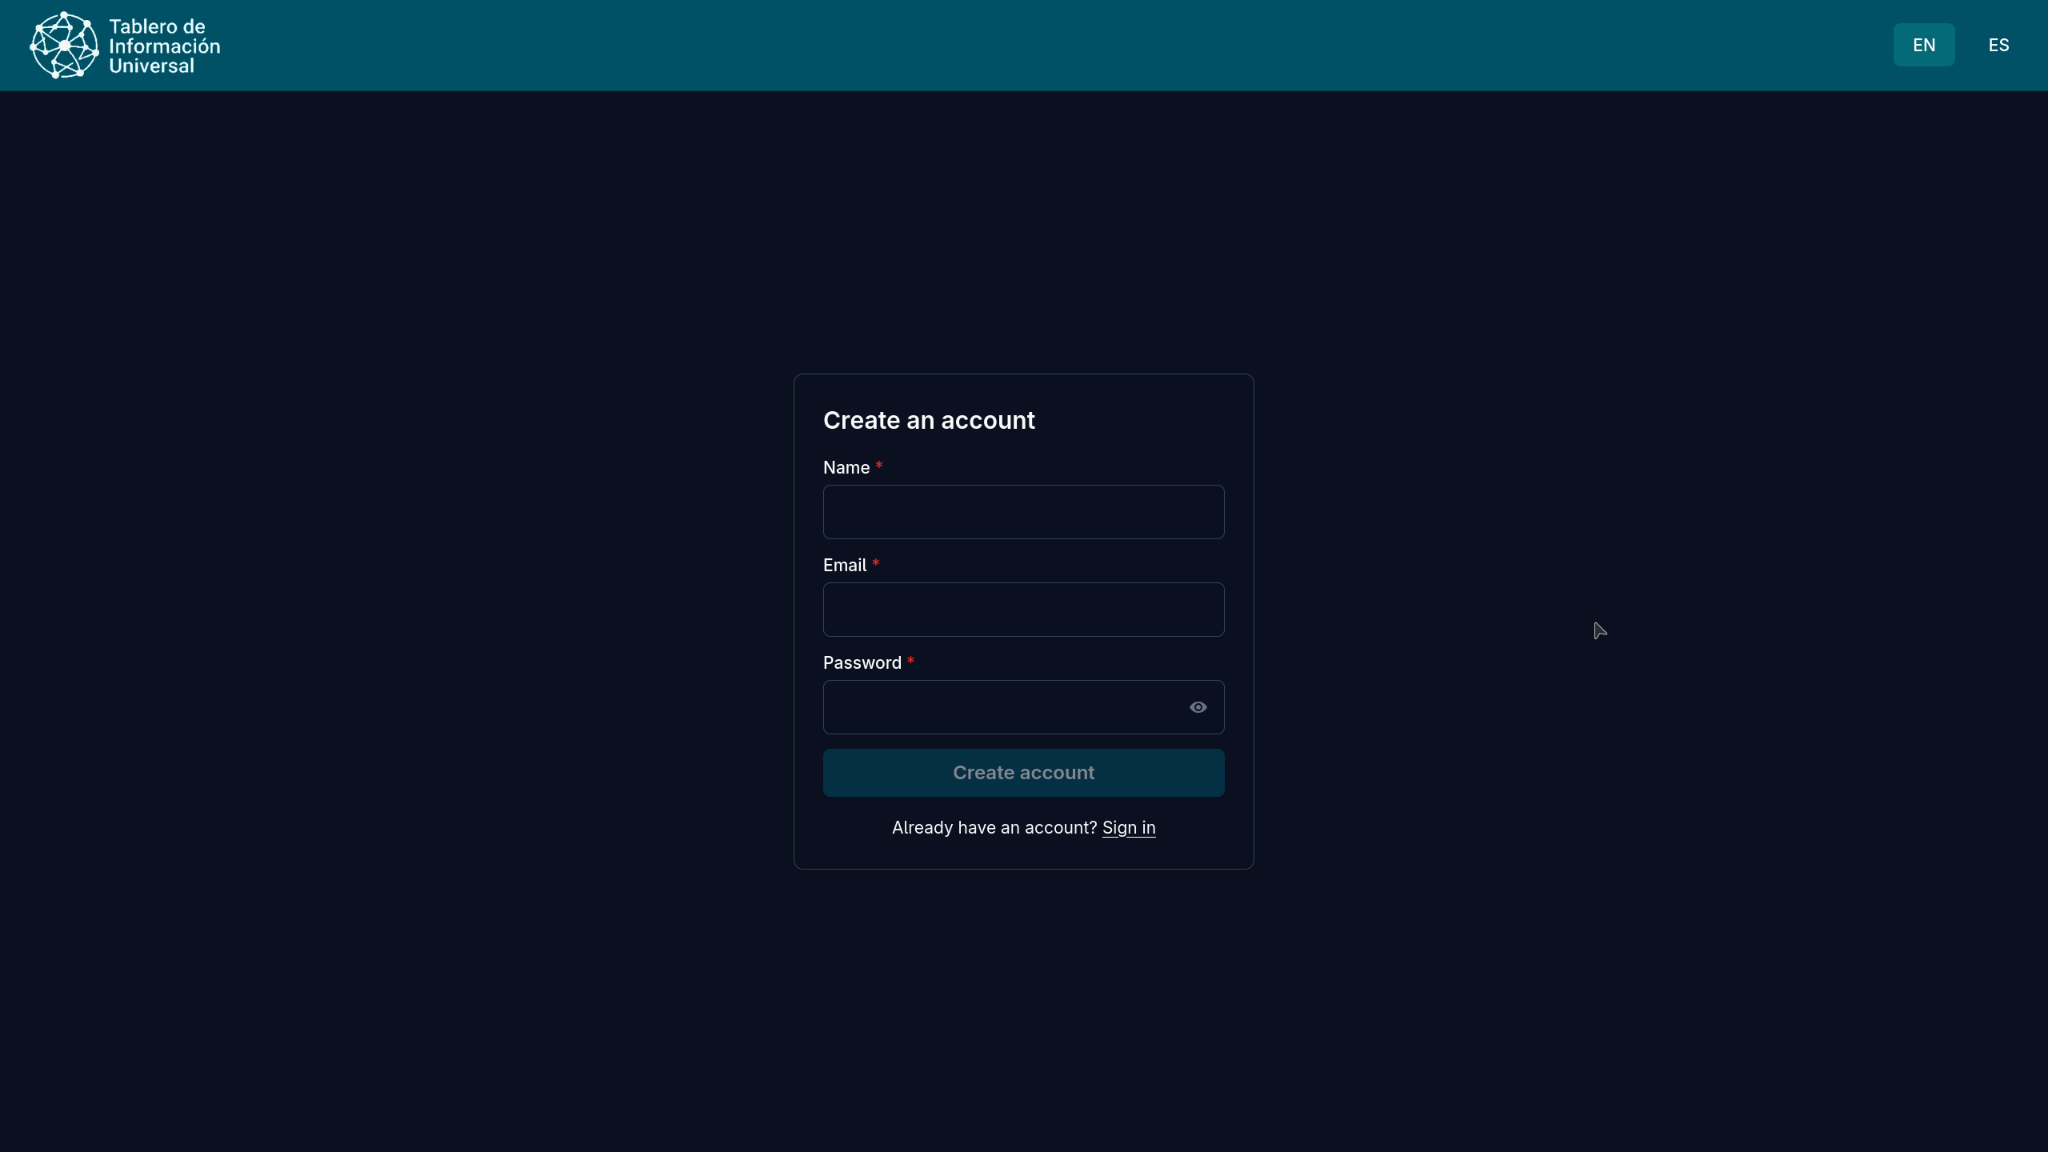
\includegraphics[width=0.92\textwidth]{figuras/fig29.png}
  \caption{Creación de cuenta}
  \label{fig:ui_registro}
\end{figure}

Una vez dentro, el usuario crea tableros desde la pantalla de inicio indicando su nombre; cada tablero nuevo pertenece a la organización seleccionada en ese momento, o al espacio personal del usuario (RF-04). La Figura~\ref{fig:ui_crear_tablero} presenta el formulario de creación.

\begin{figure}[H]
  \centering
  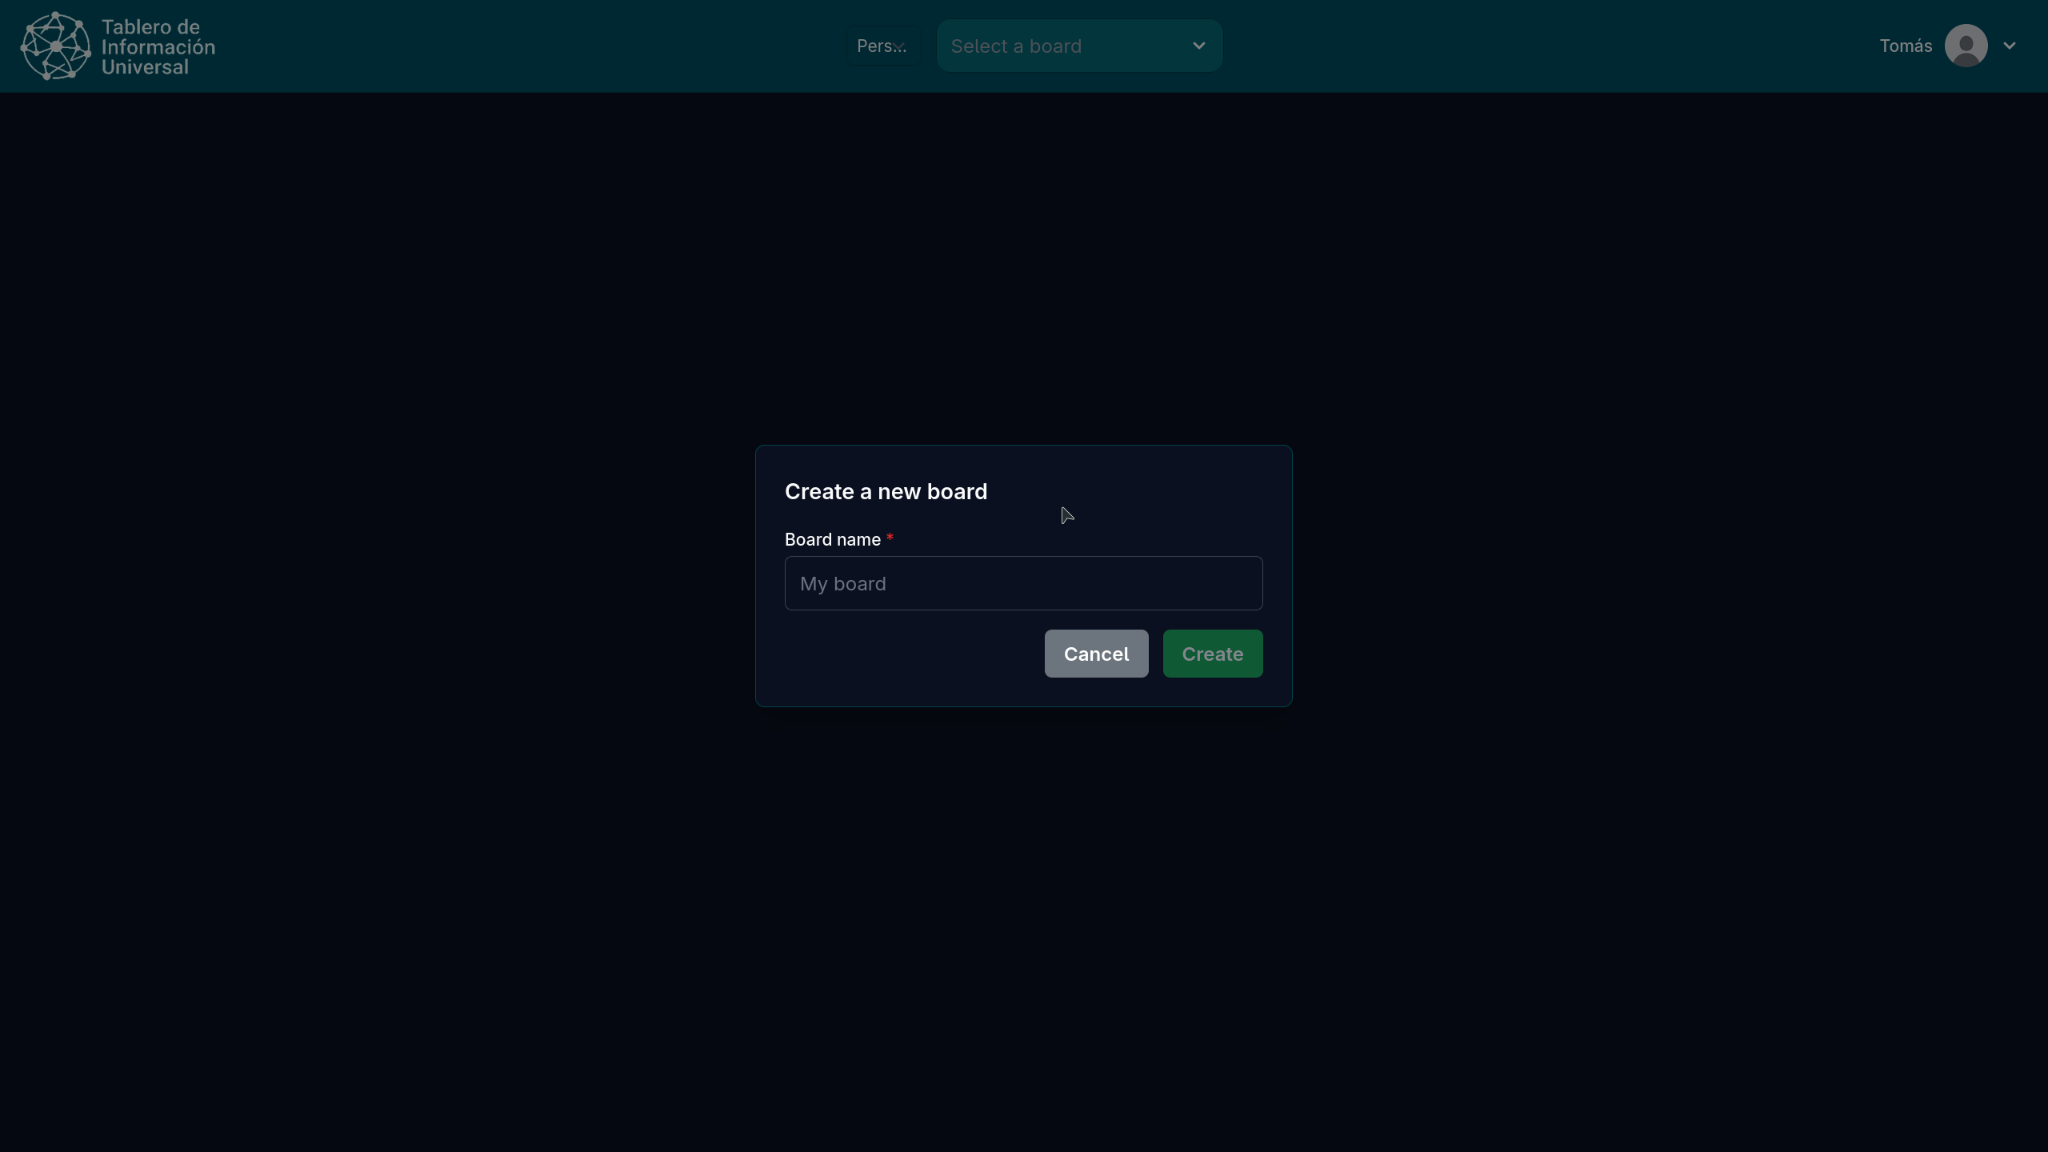
\includegraphics[width=0.92\textwidth]{figuras/fig30.png}
  \caption{Crear un tablero}
  \label{fig:ui_crear_tablero}
\end{figure}

Las tarjetas se agregan desde un carrusel que reúne las integraciones del catálogo y las plantillas disponibles en el tablero (RF-05 y RF-07). Al elegir una, el usuario completa sus variables configurables, como el repositorio en el caso de la tarjeta de GitHub, y la tarjeta se ubica en el lienzo, donde puede conectarse con otras mediante hilos (RF-06). Las Figuras~\ref{fig:ui_carrusel} a \ref{fig:ui_multiples_tarjetas} ilustran este recorrido.

\begin{figure}[H]
  \centering
  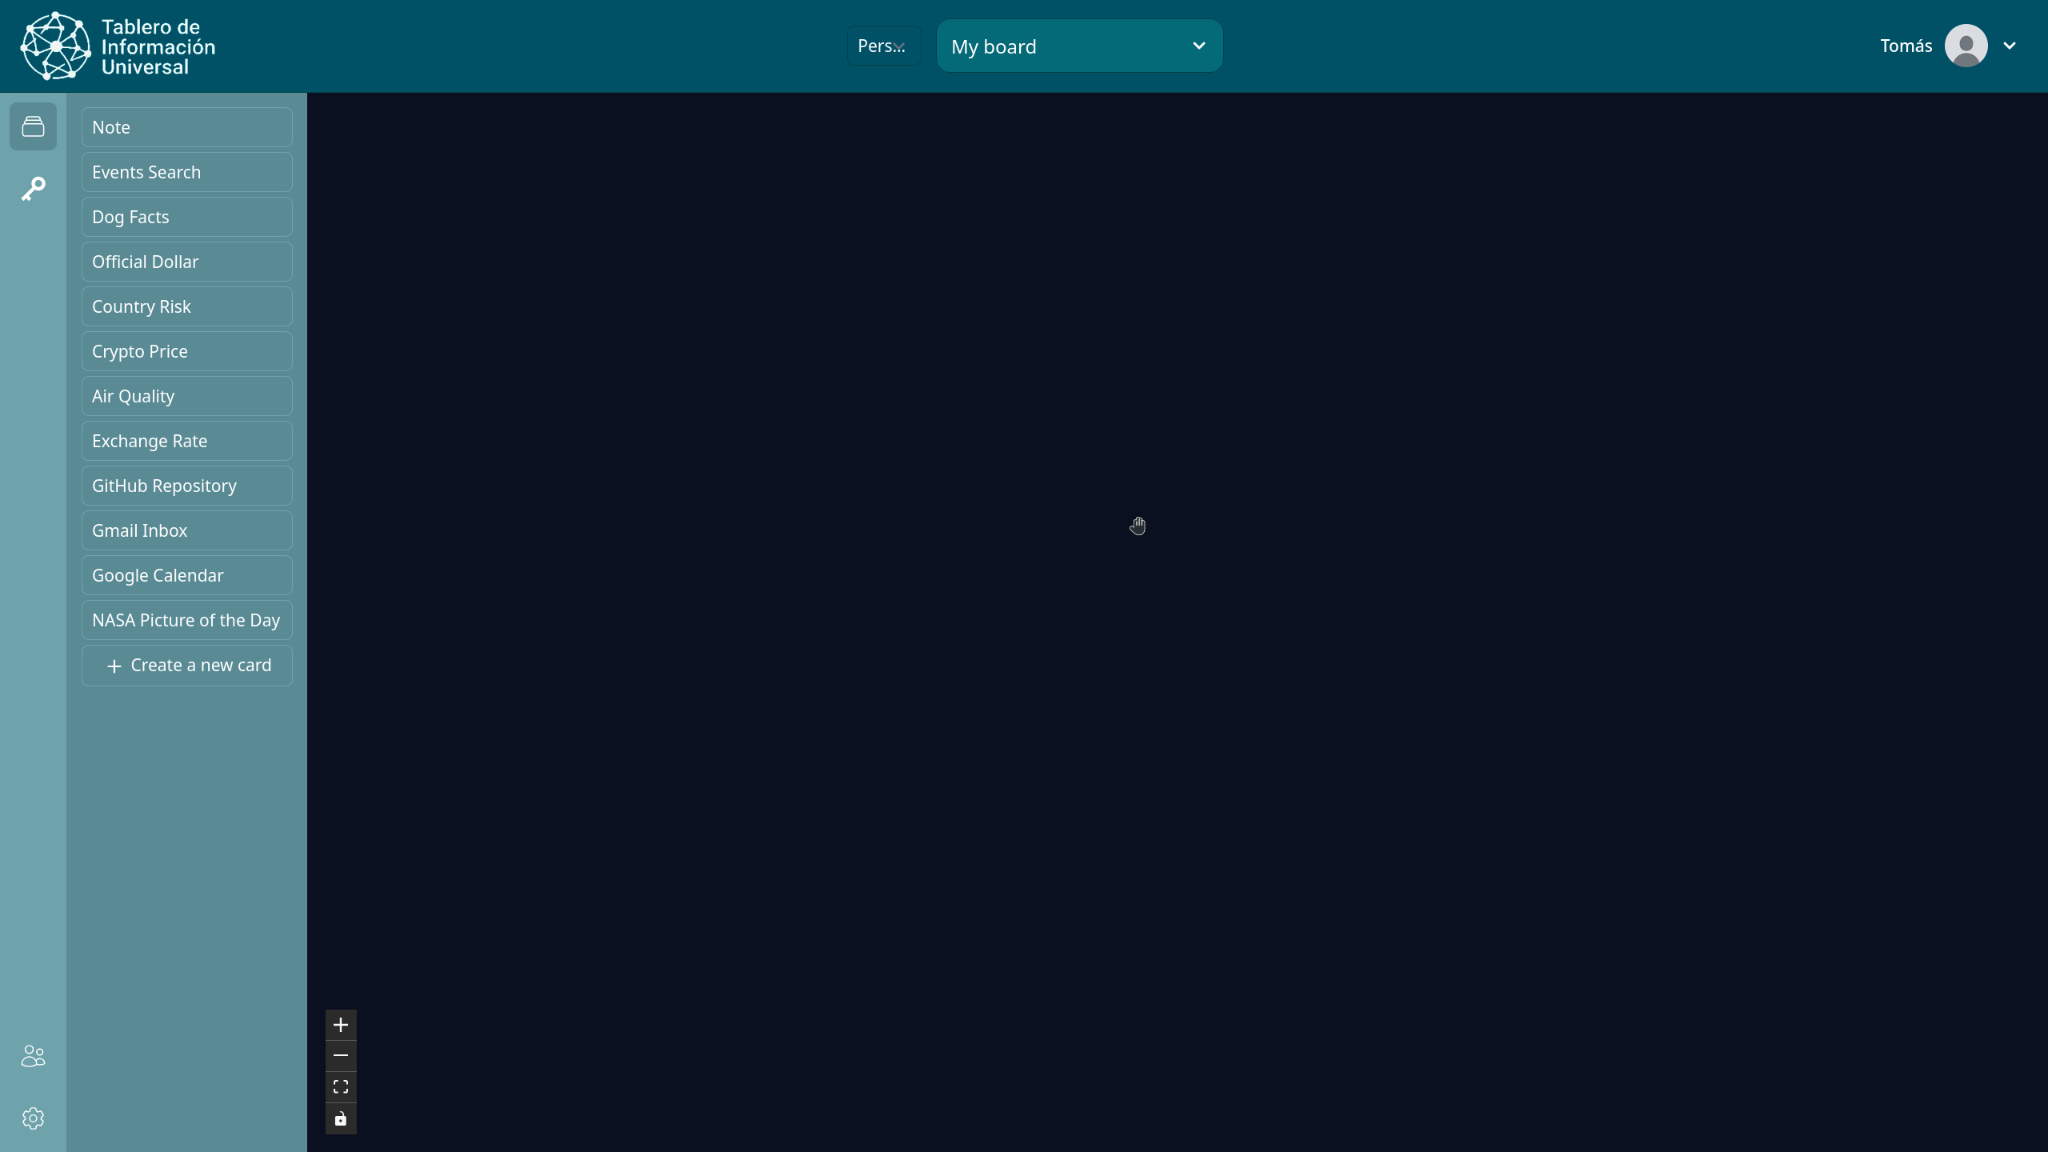
\includegraphics[width=0.92\textwidth]{figuras/fig31.png}
  \caption{Carrusel de tarjetas configurables}
  \label{fig:ui_carrusel}
\end{figure}

\begin{figure}[H]
  \centering
  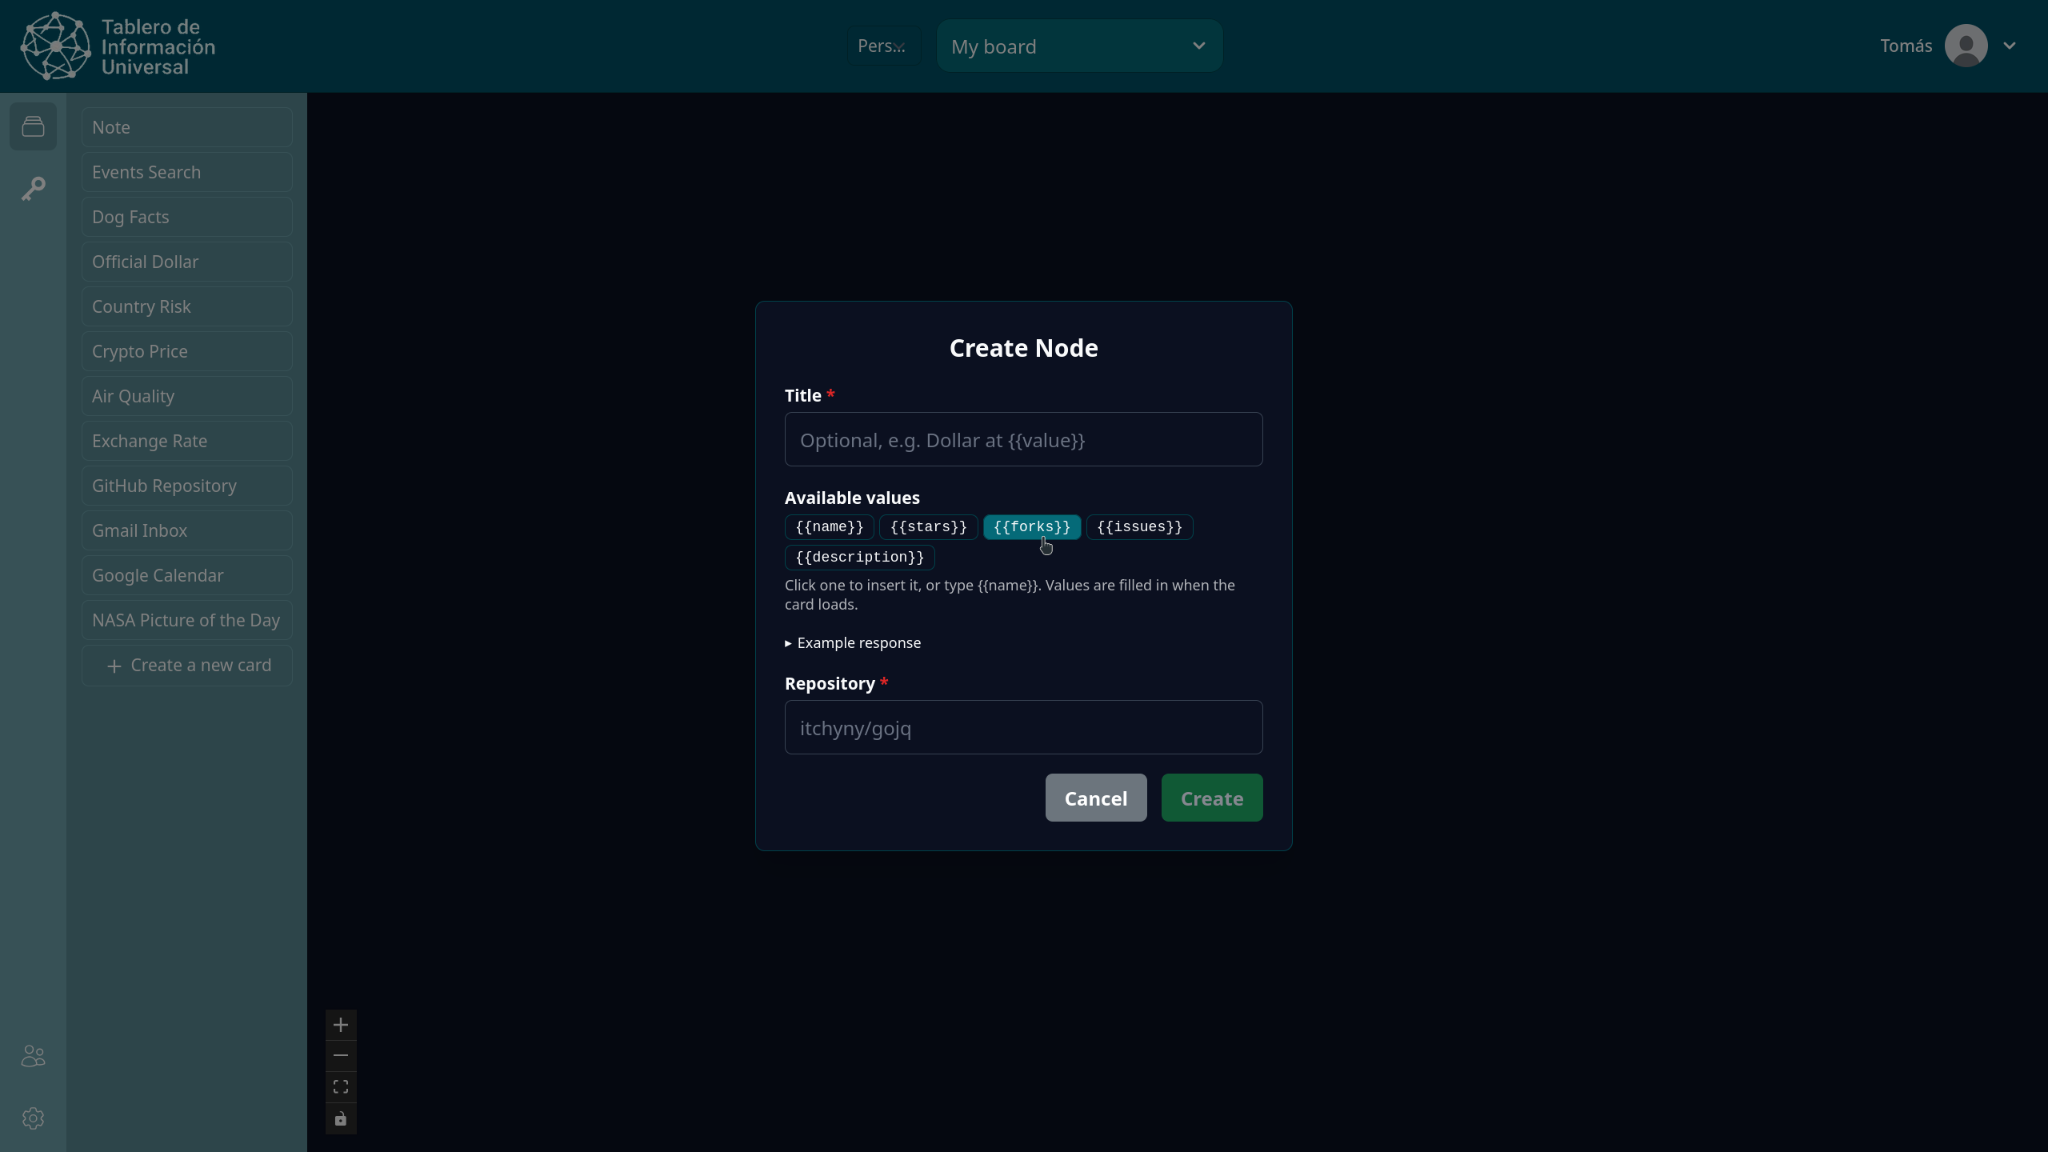
\includegraphics[width=0.92\textwidth]{figuras/fig32.png}
  \caption{Creación de tarjeta github - seleccionando variables configurables}
  \label{fig:ui_crear_github}
\end{figure}

\begin{figure}[H]
  \centering
  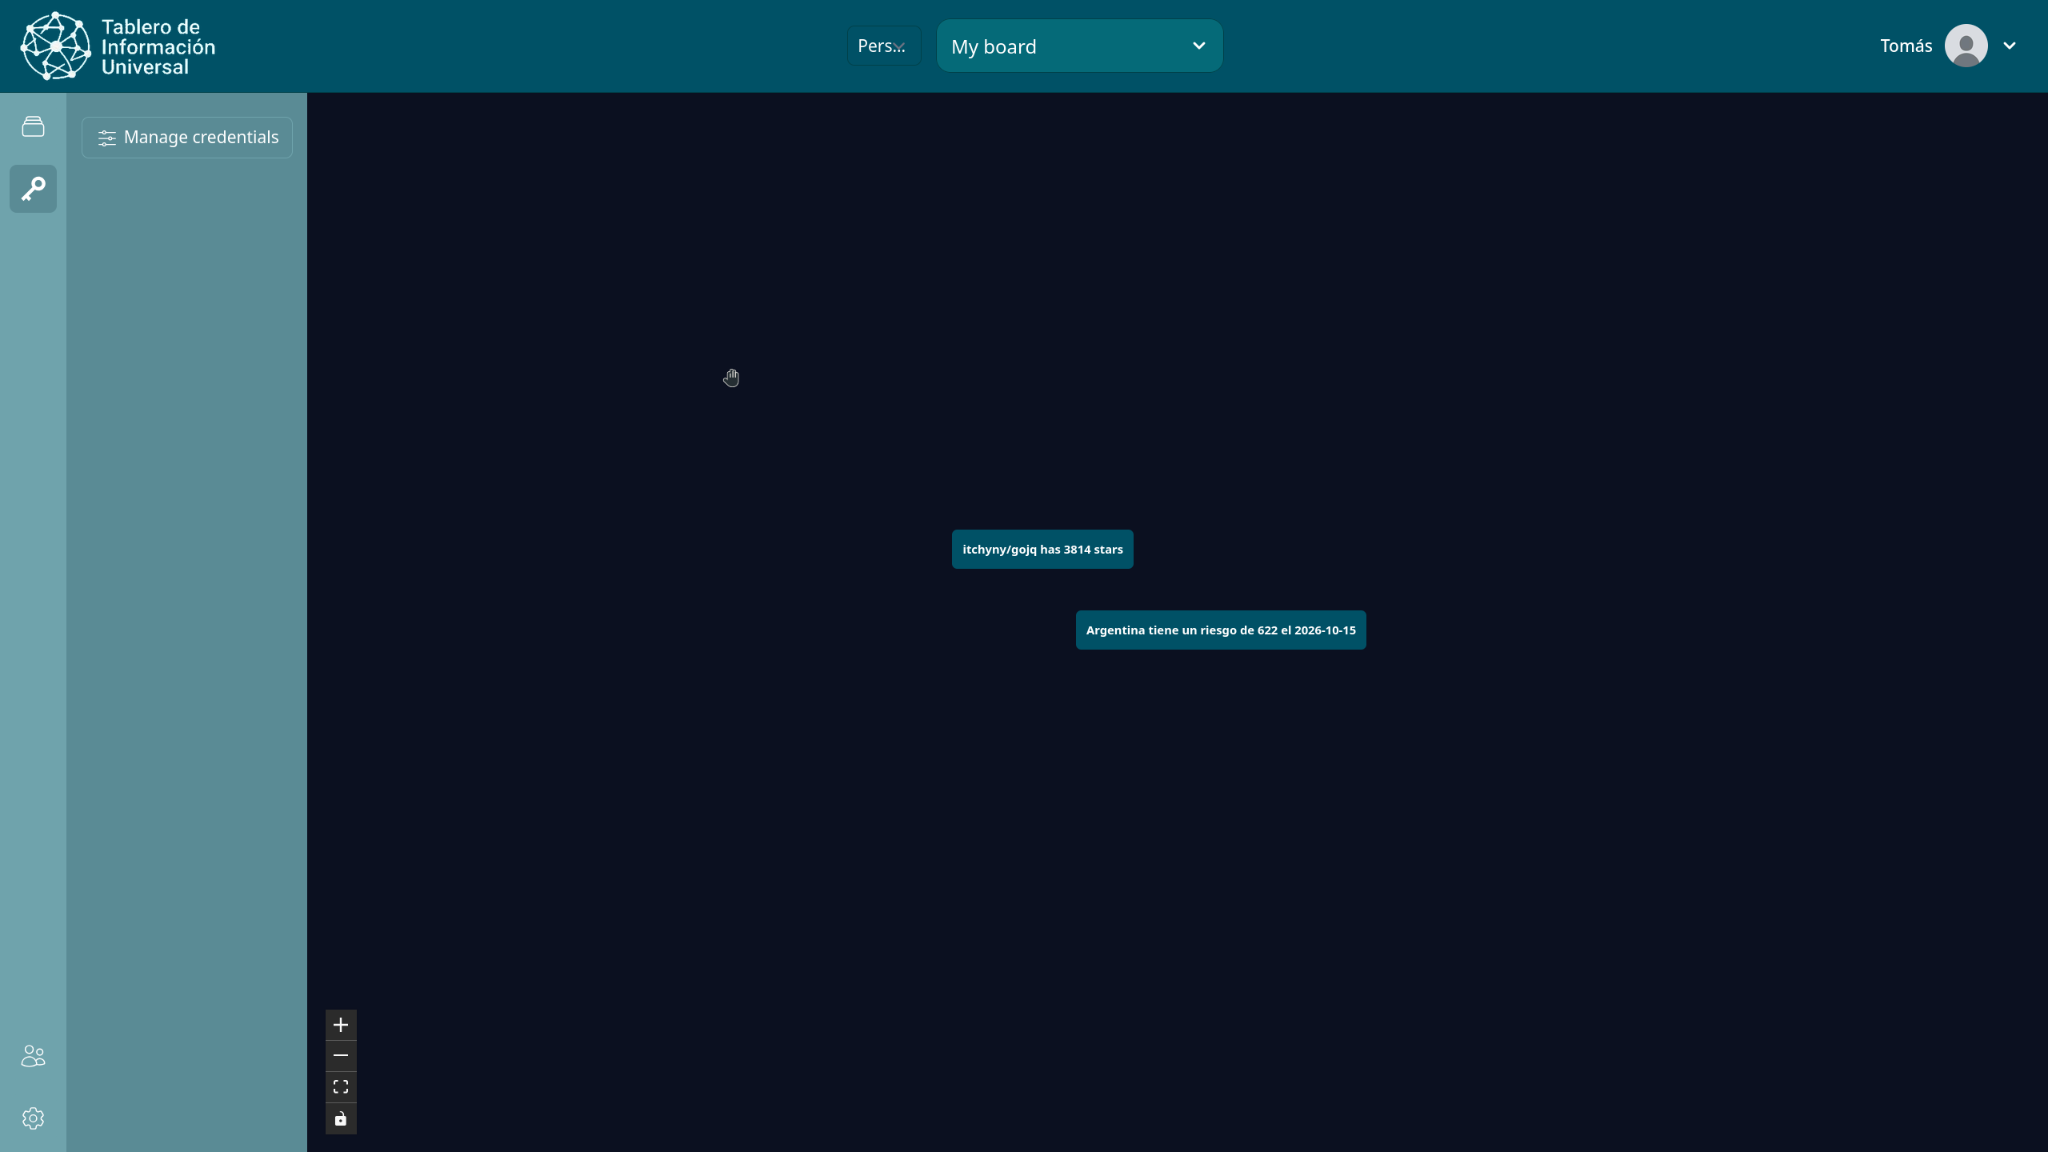
\includegraphics[width=0.92\textwidth]{figuras/fig33.png}
  \caption{Multiples tarjetas en un tablero y el carrusel de secretos}
  \label{fig:ui_multiples_tarjetas}
\end{figure}

Las integraciones que requieren autenticación toman sus credenciales del gestor de secretos del tablero, que permite cargar claves de API o conectar una cuenta externa mediante OAuth2. Al crear una tarjeta de este tipo, el formulario ofrece las credenciales que el usuario puede utilizar. Las Figuras~\ref{fig:ui_gestor_secretos} a \ref{fig:ui_nodo_credencial} muestran el gestor de secretos y la selección de una credencial.

\begin{figure}[H]
  \centering
  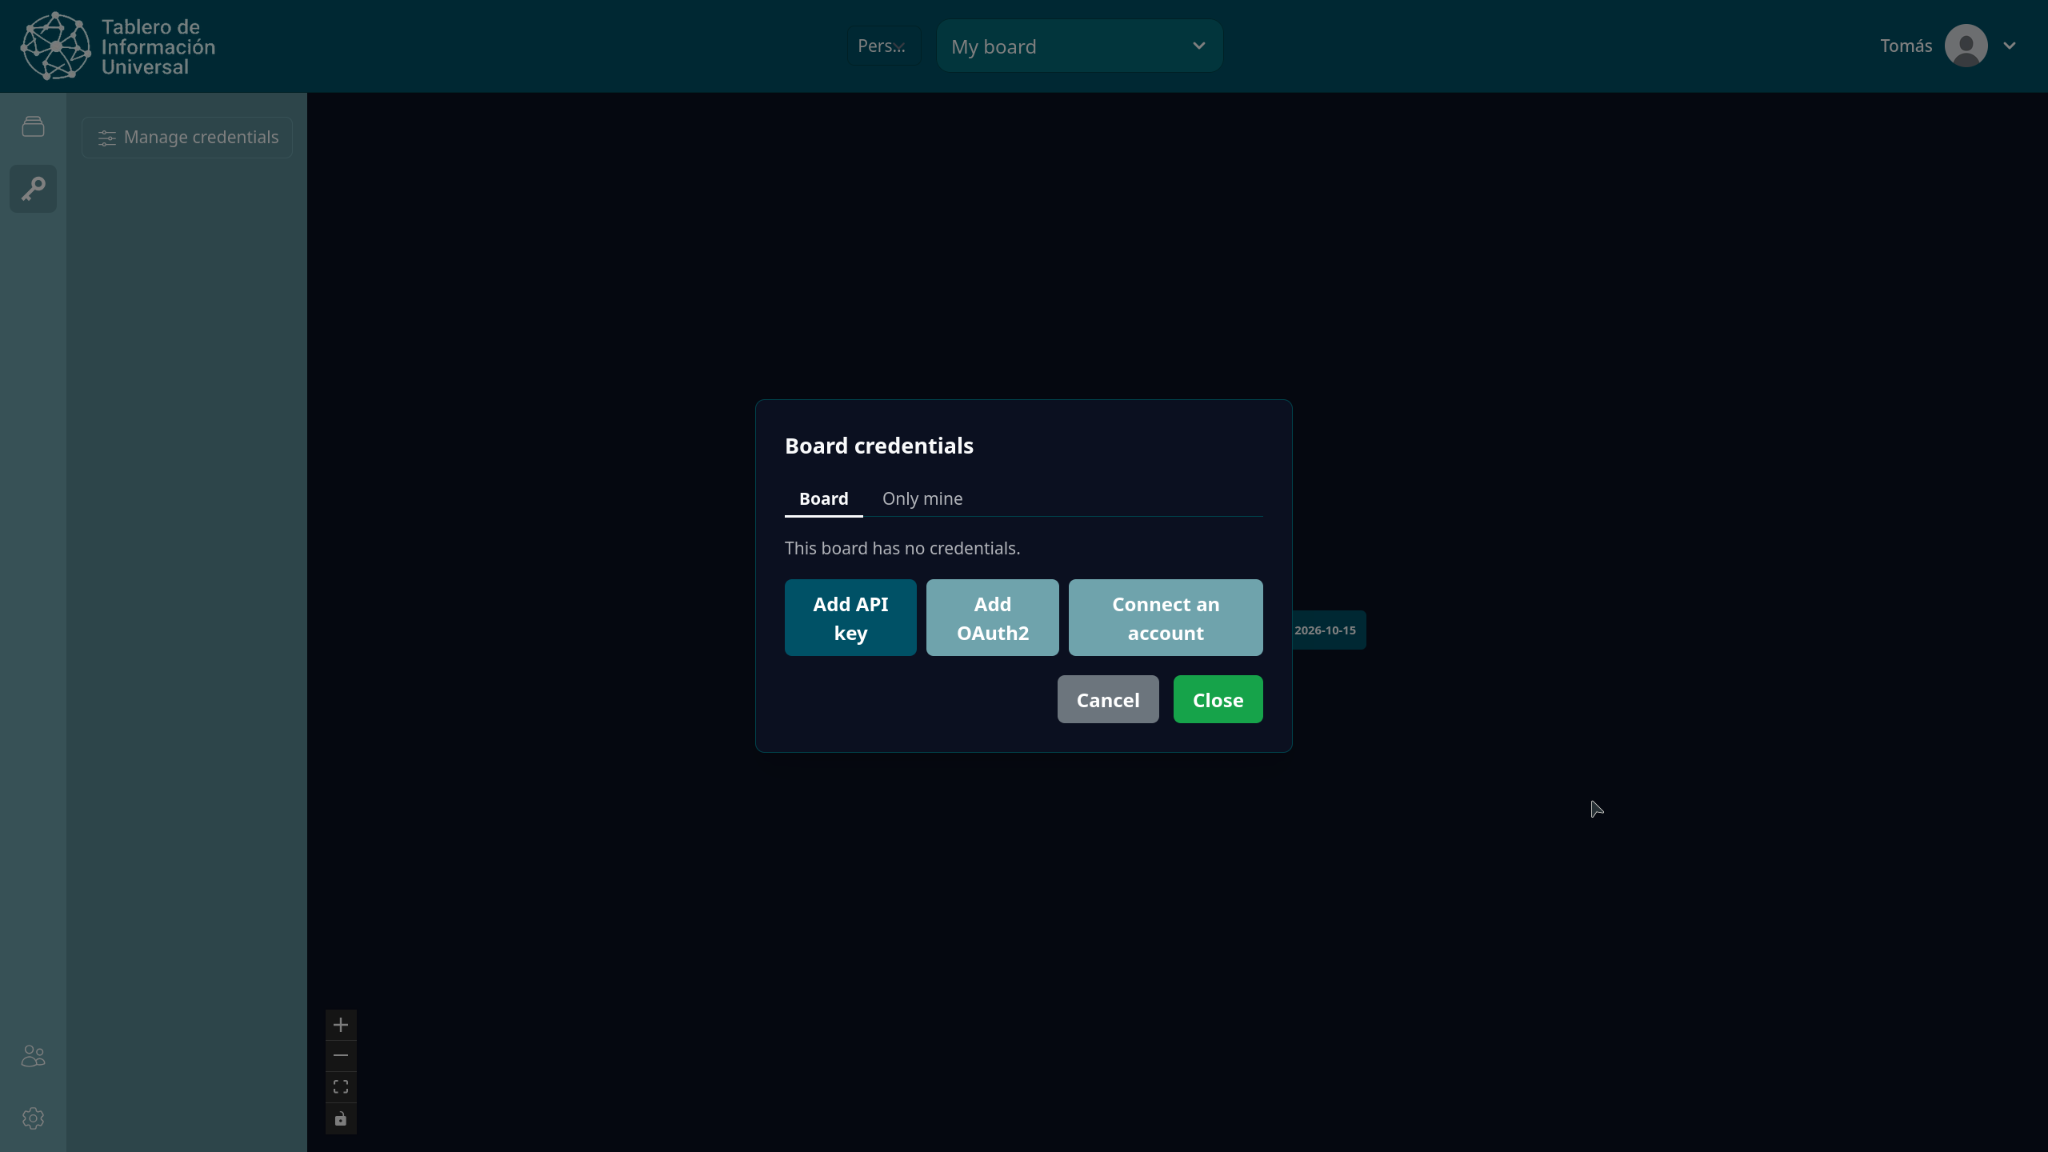
\includegraphics[width=0.92\textwidth]{figuras/fig34.png}
  \caption{Gestor de secretos del tablero}
  \label{fig:ui_gestor_secretos}
\end{figure}

\begin{figure}[H]
  \centering
  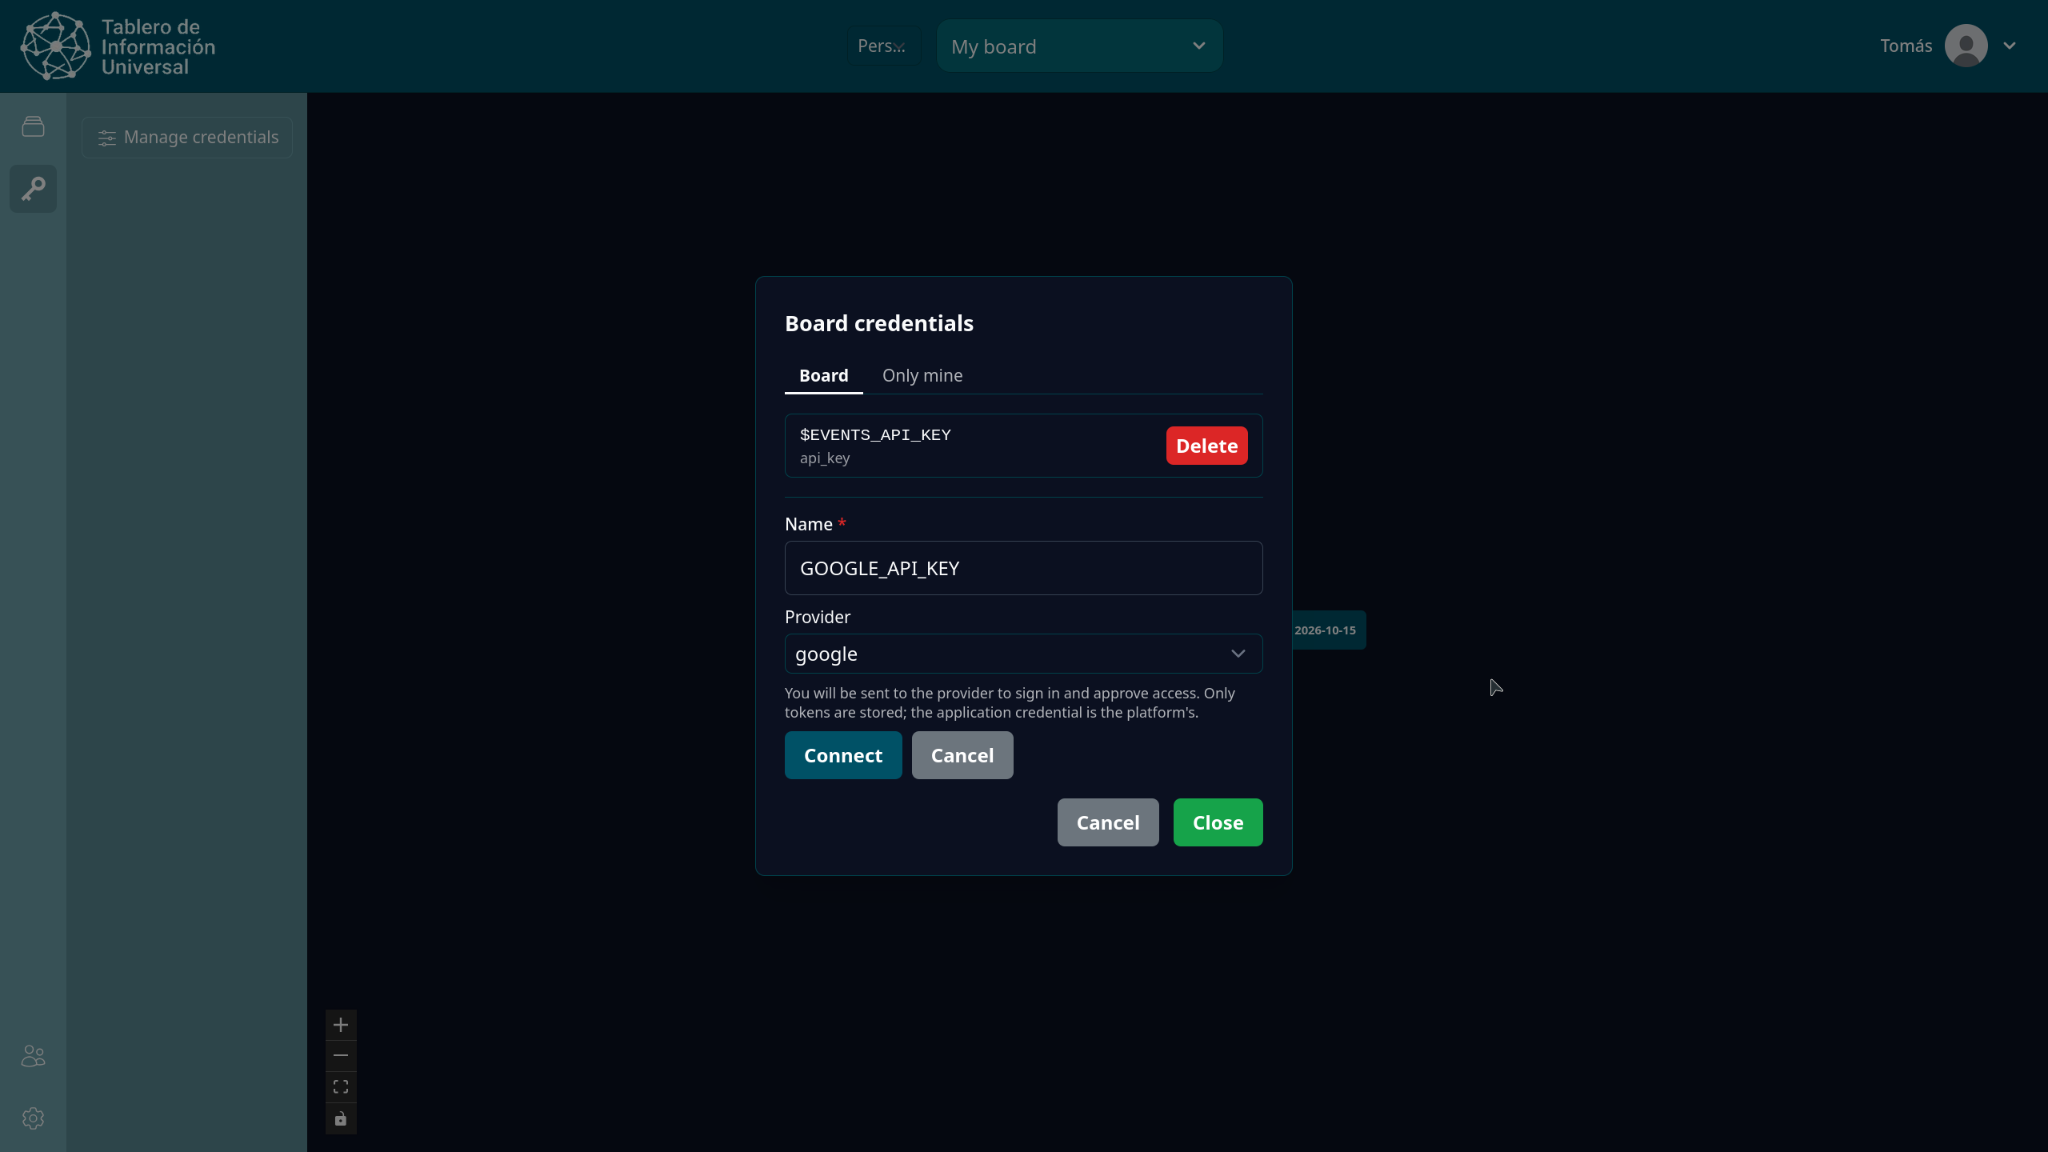
\includegraphics[width=0.92\textwidth]{figuras/fig35.png}
  \caption{Gestor de secretos, sumando una conexión OAuth}
  \label{fig:ui_oauth_secreto}
\end{figure}

\begin{figure}[H]
  \centering
  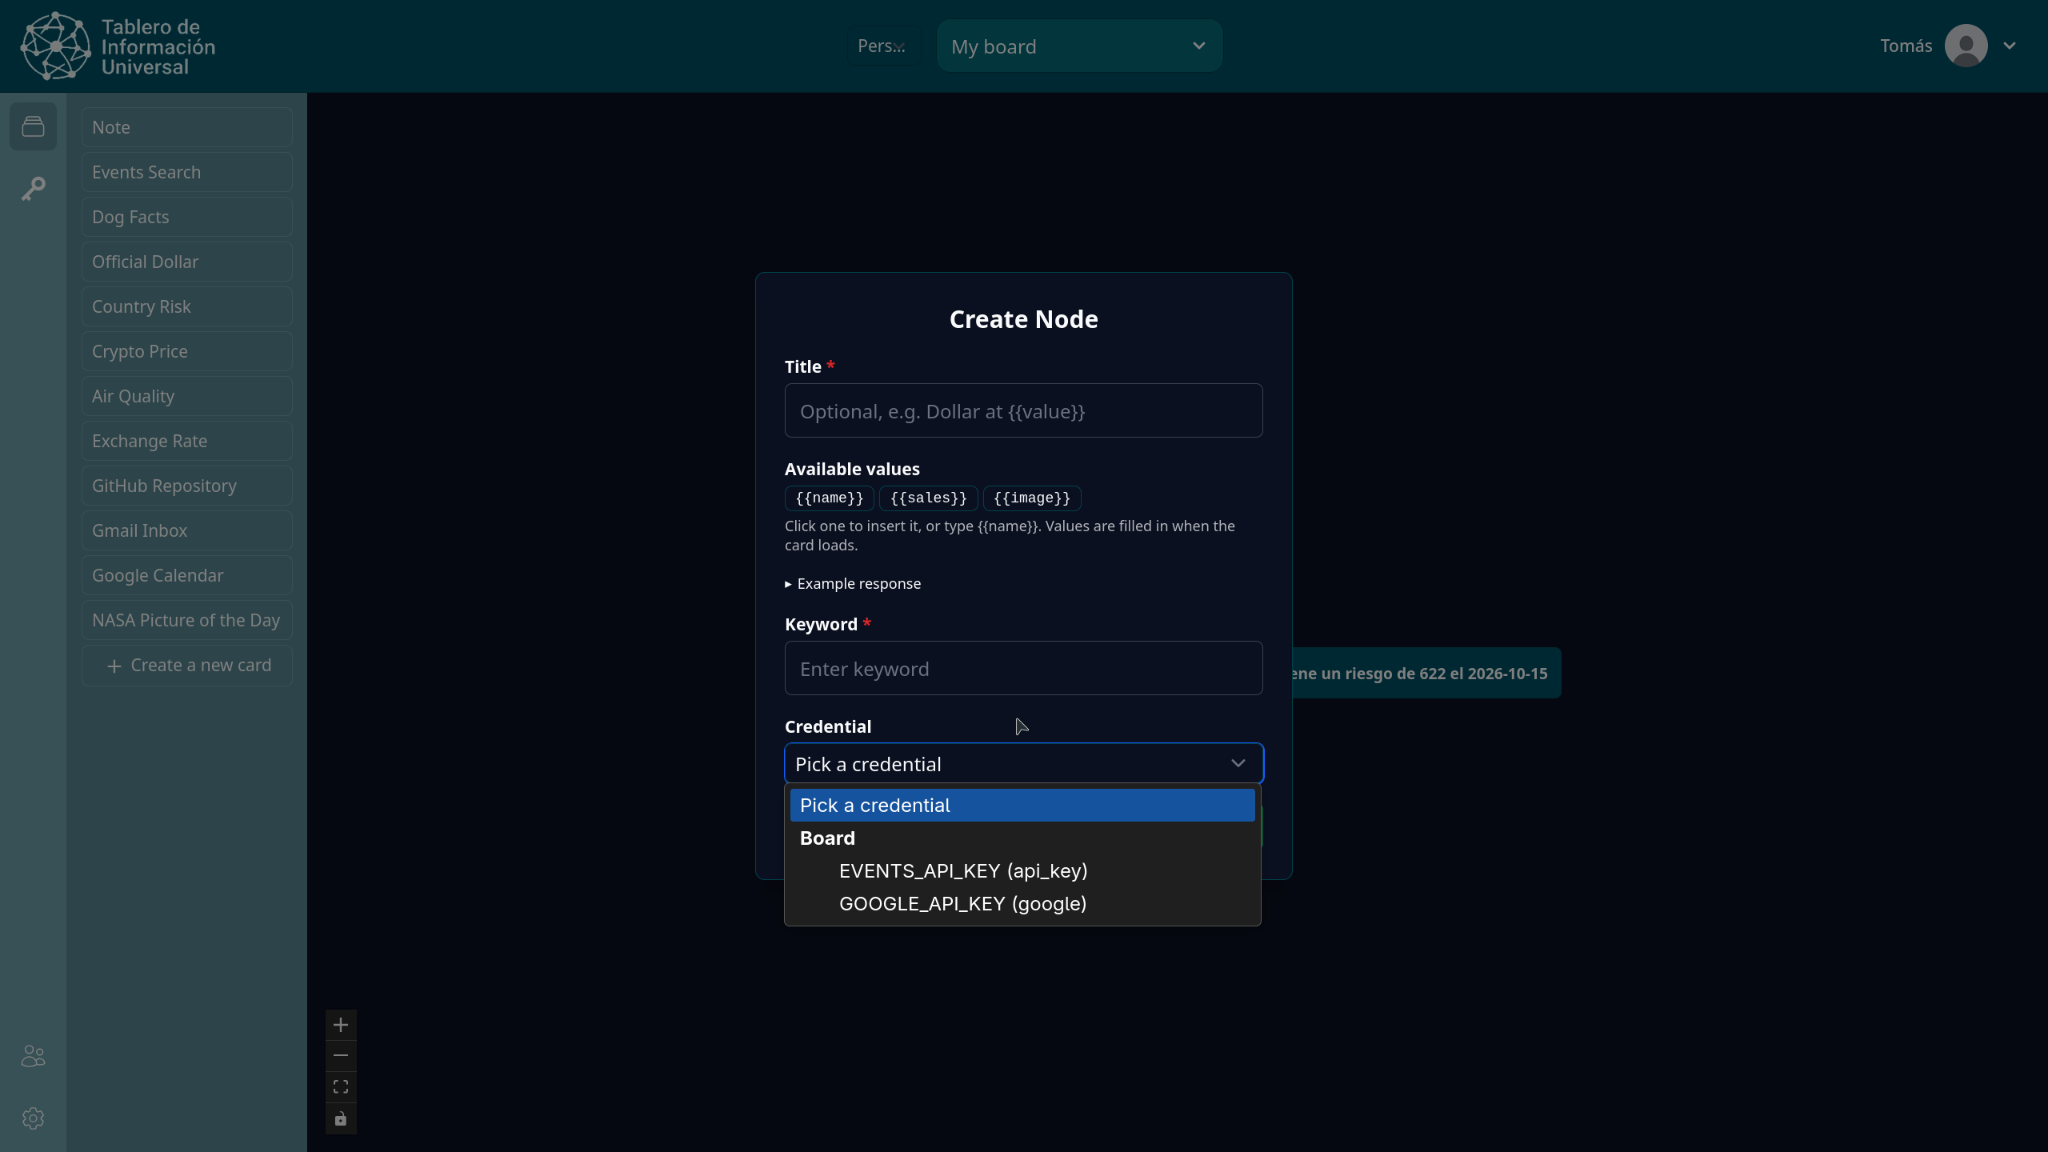
\includegraphics[width=0.92\textwidth]{figuras/fig36.png}
  \caption{Creación de nodo que requiere una credencial}
  \label{fig:ui_nodo_credencial}
\end{figure}

Por último, el dueño de un tablero puede compartirlo por email, asignando a cada persona el rol de editor o de lector (RF-13), y la pantalla de inicio reúne todos los tableros a los que el usuario tiene acceso. Desde el perfil, el usuario modifica sus datos y gestiona los tokens personales con los que se conectan herramientas externas, como el servidor MCP (RF-10). Las Figuras~\ref{fig:ui_compartir} a \ref{fig:ui_perfil} corresponden a estas pantallas.

\begin{figure}[H]
  \centering
  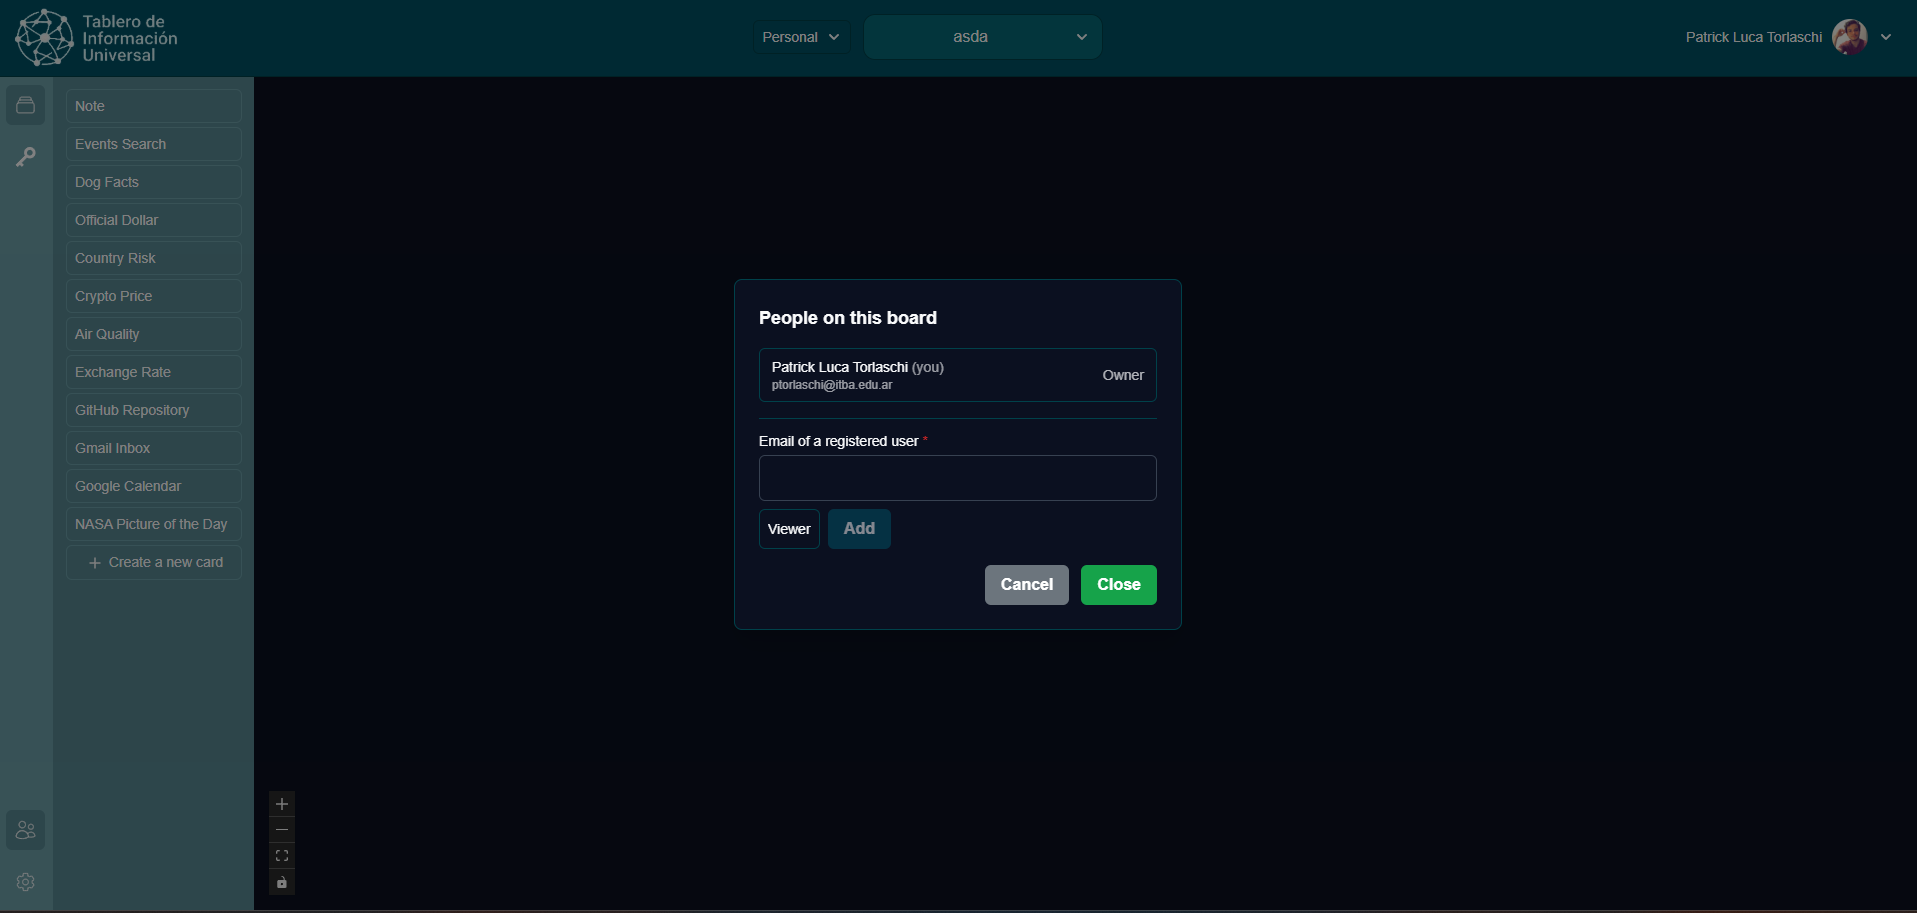
\includegraphics[width=0.92\textwidth]{figuras/fig37.png}
  \caption{Vista de compartir tablero}
  \label{fig:ui_compartir}
\end{figure}

\begin{figure}[H]
  \centering
  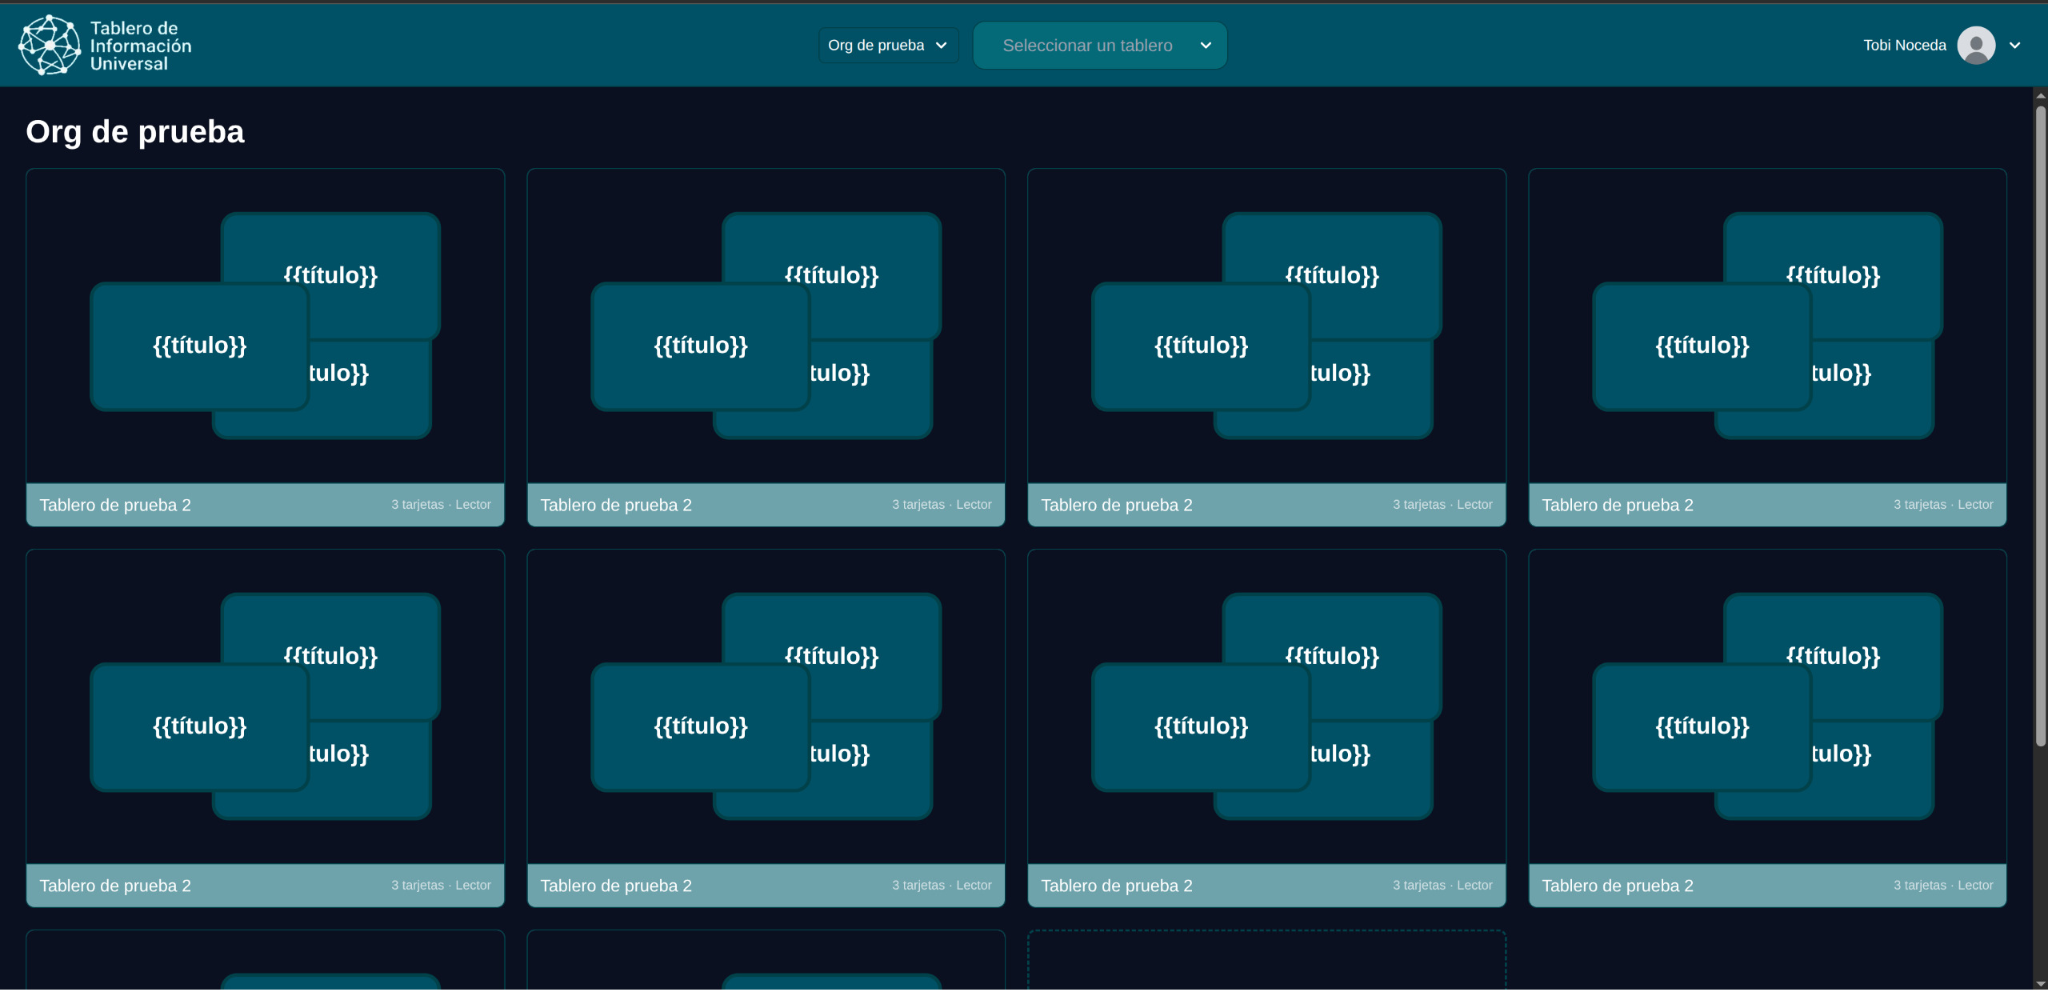
\includegraphics[width=0.92\textwidth]{figuras/fig38.png}
  \caption{Vista de inicio con varios tableros}
  \label{fig:ui_inicio_tableros}
\end{figure}

\begin{figure}[H]
  \centering
  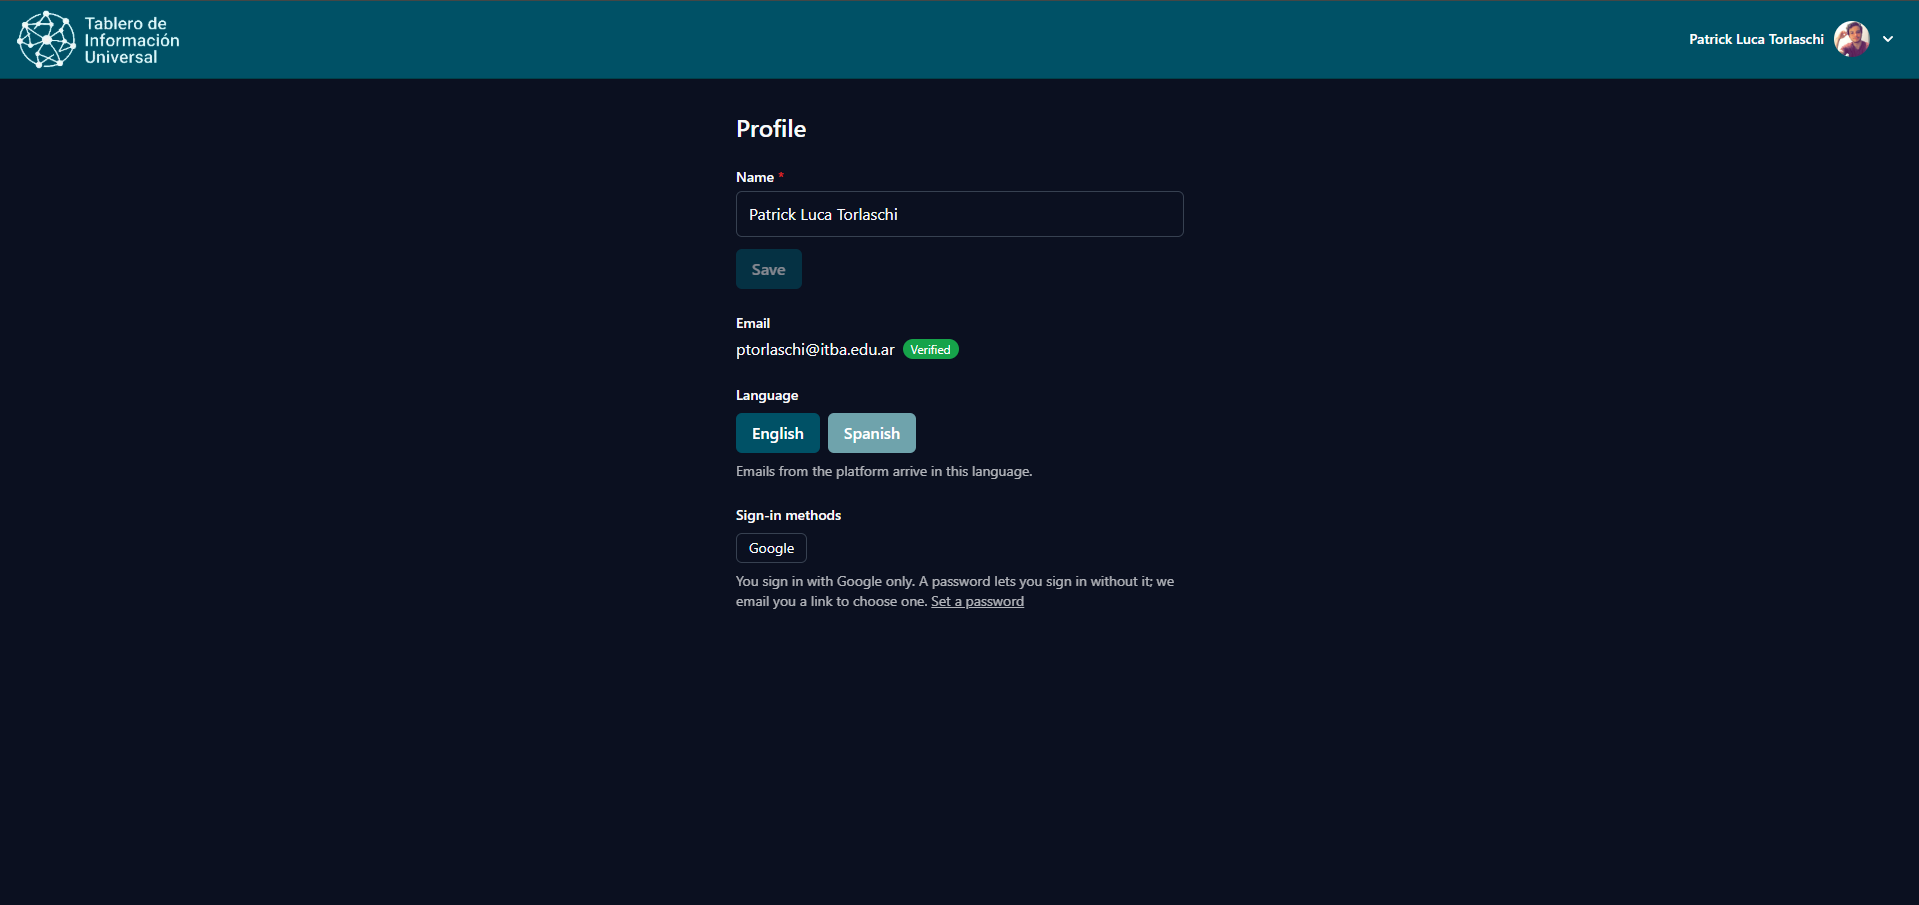
\includegraphics[width=0.92\textwidth]{figuras/fig39.png}
  \caption{Vista del perfil de usuario}
  \label{fig:ui_perfil}
\end{figure}